\documentclass{article}
\usepackage{tikz}
\usetikzlibrary{patterns,positioning,arrows,arrows.meta,calc,shapes,pgfplots.groupplots,fit,backgrounds}
\usepackage{transparent}

\begin{document}


\begin{figure*}[hb!]
    \centering
    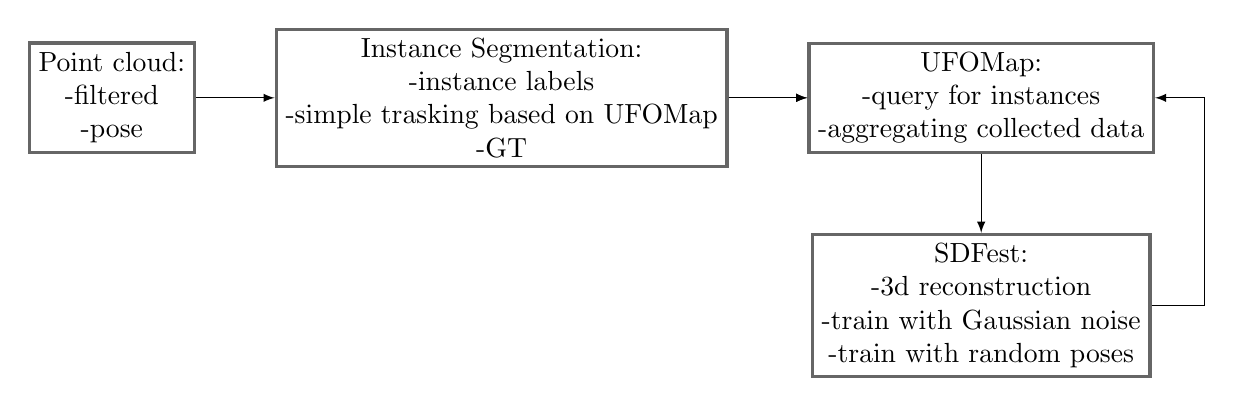
\begin{tikzpicture}[squarednode/.style={rectangle, draw=black!60,  very thick, minimum size=5mm},every text node part/.style={align=center},   dot/.style={
        % fill=blue,
        circle,
        minimum size=3pt}]
    %Nodes
    \node[squarednode]      at (-5,1.5)  (pointcloud)                              {Point cloud: \\ -filtered \\ -pose};
    
    \node[squarednode]      (instance)         [right=of pointcloud]                      {Instance Segmentation: \\ -instance labels \\-simple trasking based on UFOMap \\-GT};
    
    \node[squarednode]      (ufo)         [right=of instance]                      {UFOMap:\\-query for instances\\-aggregating collected data};
    
     \node[squarednode]      (sdf)         [below=of ufo]                      {SDFest:\\-3d reconstruction \\-train with Gaussian noise\\-train with random poses};
        %Lines
    \draw[-latex] (pointcloud.east) -- (instance.west);
    \draw[-latex] (instance.east) -- (ufo.west);
    \draw[-latex] (instance.east) -- (ufo.west);
    \draw[-latex] (ufo.south) -- (sdf.north);
    \draw[-latex] (sdf.east) -| ($(sdf.west) + (5,0mm)$) |- (ufo.east);
    % \draw[-latex] (sdf.east) |- (ufo.east);


    \end{tikzpicture}
        \caption{}
        \label{fig:pipeline}
\end{figure*}

\end{document}
